\chapter{Nodo estandar de red}
	\label{chap:nodo_de_red}

El \smallcaps{nodo de red} es el elemento central del acelerador en hardware basado en múltiples núcleos. Cada nodo consta de un router, una interfaz de red y un elemento de procesamiento. La figura \ref{fig:ch4_nodo} muestra un diagrama a bloques de un nodo general. El diseño modular de los nodos permite la actualización de la lógica en cada miembro del sistema de manera independiente, sin requerir la intervencion en otros bloques del nodo.

\begin{figure}
	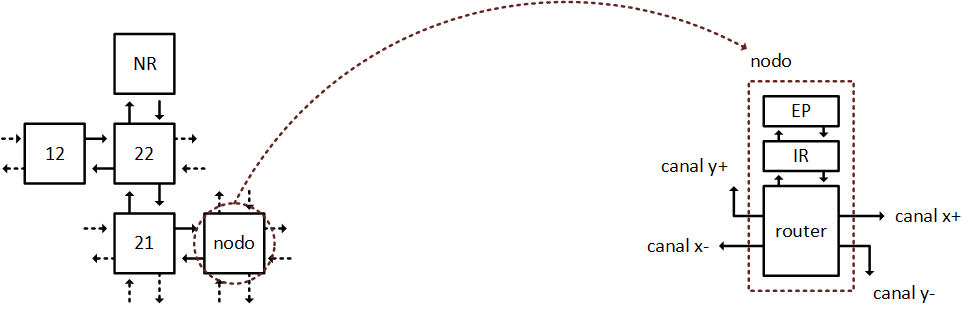
\includegraphics[width=\linewidth]{figures/ch4_nodo.png}
	\caption
		{	
			Cada nodo de red es una isla de procesamiento en el acelerador. Las líneas de interconexión entre nodos se denominan canales. EP: Elemento de procesamiento, IR: Interfaz de red
		}
	\label{fig:ch4_nodo}
\end{figure}

La operación de un nodo de red puede resumirse de la siguiente manera: Un paquete en tránsito ingresa por cualquiera de los canales de entrada del nodo para ser procesado por el modulo router. Dentro del router se determina si el paquete en tránsito ya ha sido procesado de manera previa en otro nodo a lo largo de su camino. En caso de que un paquete haya sido recibido de manera previa por otro elemento de procesamiento, este se envía en dirección a una puerta de salida de la red para ser recolectado, en caso contrario, se lleva a cabo una solicitud de ingreso al elemento de procesamiento del nodo. Si el elemento de procesamiento se encuentra disponible el paquete ingresa a el para el procesamiento del mensaje. En caso que el elemento de procesamiento se encuentre atendiendo otra petición, el router verifica si algún otro puerto de salida productivo para el tránsito del paquete se encuentra disponible, de así serlo, el paquete se transfiere a ese puerto para que continúe su búsqueda por un elemento de procesamiento disponible en otro nodo de la red.

El capítulo se desarrolla en el siguiente orden: La siguiente sección presenta el formato de paquete utilizado para organizar los datos previo a su transferencia entre nodos de la red. Los campos que forman un paquete, así como su organización, determinan el comportamiento y micro-arquitectura del router. De manera posterior, se presenta a detalle la organización interna del router así como su funcionamiento. En la parte final del capítulo se presenta la arquitectura de una interfaz de red minimalista para los nodos de red. El desarrollo de interfaces de red para diferentes elementos de procesamiento se discute en esta seccion dando como ejemplo una interfaz para un encriptador basado en el algoritmo \textit{DES} \cite{chapter0:NIST:1977:DES}.


\section{Formato de paquete}
	\label{sec:formato_paquete}

Los elementos de procesamiento trabajan con bloques de datos de longitud fija. Al tener un tamaño predeterminado el formato de paquete se simplifica, eliminando secciones destinadas al control de flujo de datagramas de longitud variable. Un beneficio extra del uso de paquetes simples es la reducción en la lógica necesaria para la decodificación de los mismos.


\begin{figure}
	\begin{center}
		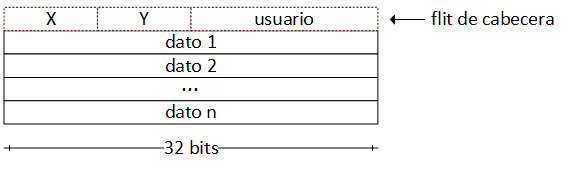
\includegraphics[scale=0.7]{figures/ch4_organizacion_paquete.png}
	\end{center}
	\caption
		{	
			No existe una restricción en el número de flits para el transporte de información dentro de un paquete, sin embargo, el incremento de estas unidades de transporte acarrea consigo una mayor congestión en la red, además de un incremento en la cantidad de almacenamiento temporal requerido por cada uno de los puertos del encaminador.
		}
	\label{fig:ch4_organizacion_paquete}
\end{figure}


 Todos los paquetes están formados por un flit de cabecera seguido de cualquier número de flits para el transporte de datos. El número de flits que conforman un paquete está determinado por la aplicación, y debe de especificarse de manera previa a la síntesis del acelerador. El tamaño de paquete definido en tiempo pre-síntesis hace innecesario la inclusión de un flit de final de paquete.

El contenido de los flit de datos es transparente para los nodos del sistema, los routers e interfaces de red no tienen mecanismos para la discriminación de campos o formatos dentro de ellos. El flit de cabecera es un caso particular, en el, el número y longitud de campos es fijo y tienen un profundo impacto en el funcionamiento de la lógica de los routers. La figura \ref{fig:ch4_flit_cabecera} muestra la distribución de campos a lo largo de un flit de cabecera.


\begin{figure}
	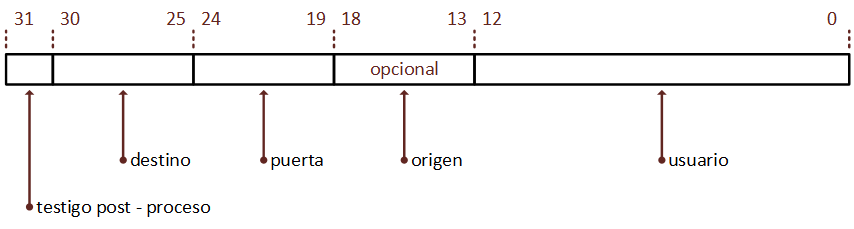
\includegraphics[width=\linewidth]{figures/ch4_flit_cabecera.png}
	\caption
		{	
			Formato de flit de cabecera. El uso del campo \textit{origen} permite la implementación de algoritmos de encaminamiento basados en el modelo \textit{odd-even}. En caso de omitir el uso del campo origen durante el proceso de planificación de ruta, su espacio puede anexarse al campo \textit{número de secuencia} para ampliar su longitud.
		}
	\label{fig:ch4_flit_cabecera}
\end{figure}

 El campo \textit{identificador de cabecera} indica la presencia de un nuevo paquete en tránsito. Una vez que un paquete a sido trabajado por un elemento de procesamiento, el campo \textit{testigo post-proceso} es activado para indicar que el paquete está en busca de una puerta de salida de la red, y no requiere competir por el uso de un elemento de procesamiento. Los campos \textit{destino}, \textit{puerta} y \textit{origen} almacenan una dirección de nodo formada por una dupla \{\textit{x,y}\}. Estos campos tienen una longitud fija de 6 bits. La distribución de bits de los campos para la representación de direcciones puede variar dependiendo de la geometría de la red, por ejemplo, se puede asignar un mayor número de bits a la dimensión \textit{x} en caso que se desee una geometría rectangular en lugar de una cuadrada. El uso de 6 bits como espacio de direcciones permite tener en la red un máximo de 64 nodos. Es posible extender el espacio de direccionamiento sacrificando capacidad de almacenamiento de los campos, \textit{número de secuencia} y textit{origen}, para extender de manera efectiva las direcciones que pueden representarse por medio de los campos destino y puerta.

El campo \textit{número de secuencia} ofrece la posibilidad de implementar mecanismos de \textit{Calidad de Servicio (QoS)}. Un ejemplo del uso de este campo es la verificación de recepción de todos los paquetes liberados a la red para su procesamiento. En el escenario anterior, el campo número de secuencia es utilizado para incluir un identificador a cada paquete, mediante este número se puede corroborar que todos los paquetes liberados para procesamiento en la red han sido recibidos en en la puerta de salida correcta. Los servicios \textit{QoS} pueden implementarse directamente en hardware o software dependiendo de la interfaz para la extracción de datos del acelerador.


\section{Router}\label{sec:router}

La arquitectura del router está definida para operar bajo el esquema de conmutación de paquetes utilizando la técnica \textit{virtual cut-through}. La estrategia para el control de flujo se basa en el uso de \textit{créditos} entre routers de la red. El diseño permite definir de manera previa a la síntesis el ancho de canales de entrada/salida y la capacidad de almacenamiento temporal para paquetes entrando al encaminador (tamaño de \textit{buffers}).

De manera interna un router está organizado en dos particiones lógicas, una dedicada al transporte de datos y una segunda partición para el control de la dirección en la que la información fluye a través del módulo. El camino que debe de seguir un paquete en transito a traves del router incluye los siguientes bloques: una \textit{cola de almacenamiento} temporal o \textit{buffer}, la estructura de interconexión entre puertos del encaminador, y un registro de salida. El conjunto de bloques mencionado anteriormente se conoce como camino de datos. La figura \ref{fig:ch4_top_level_router} muestra un diagrama a bloques de alto nivel de un router.


\begin{figure}
	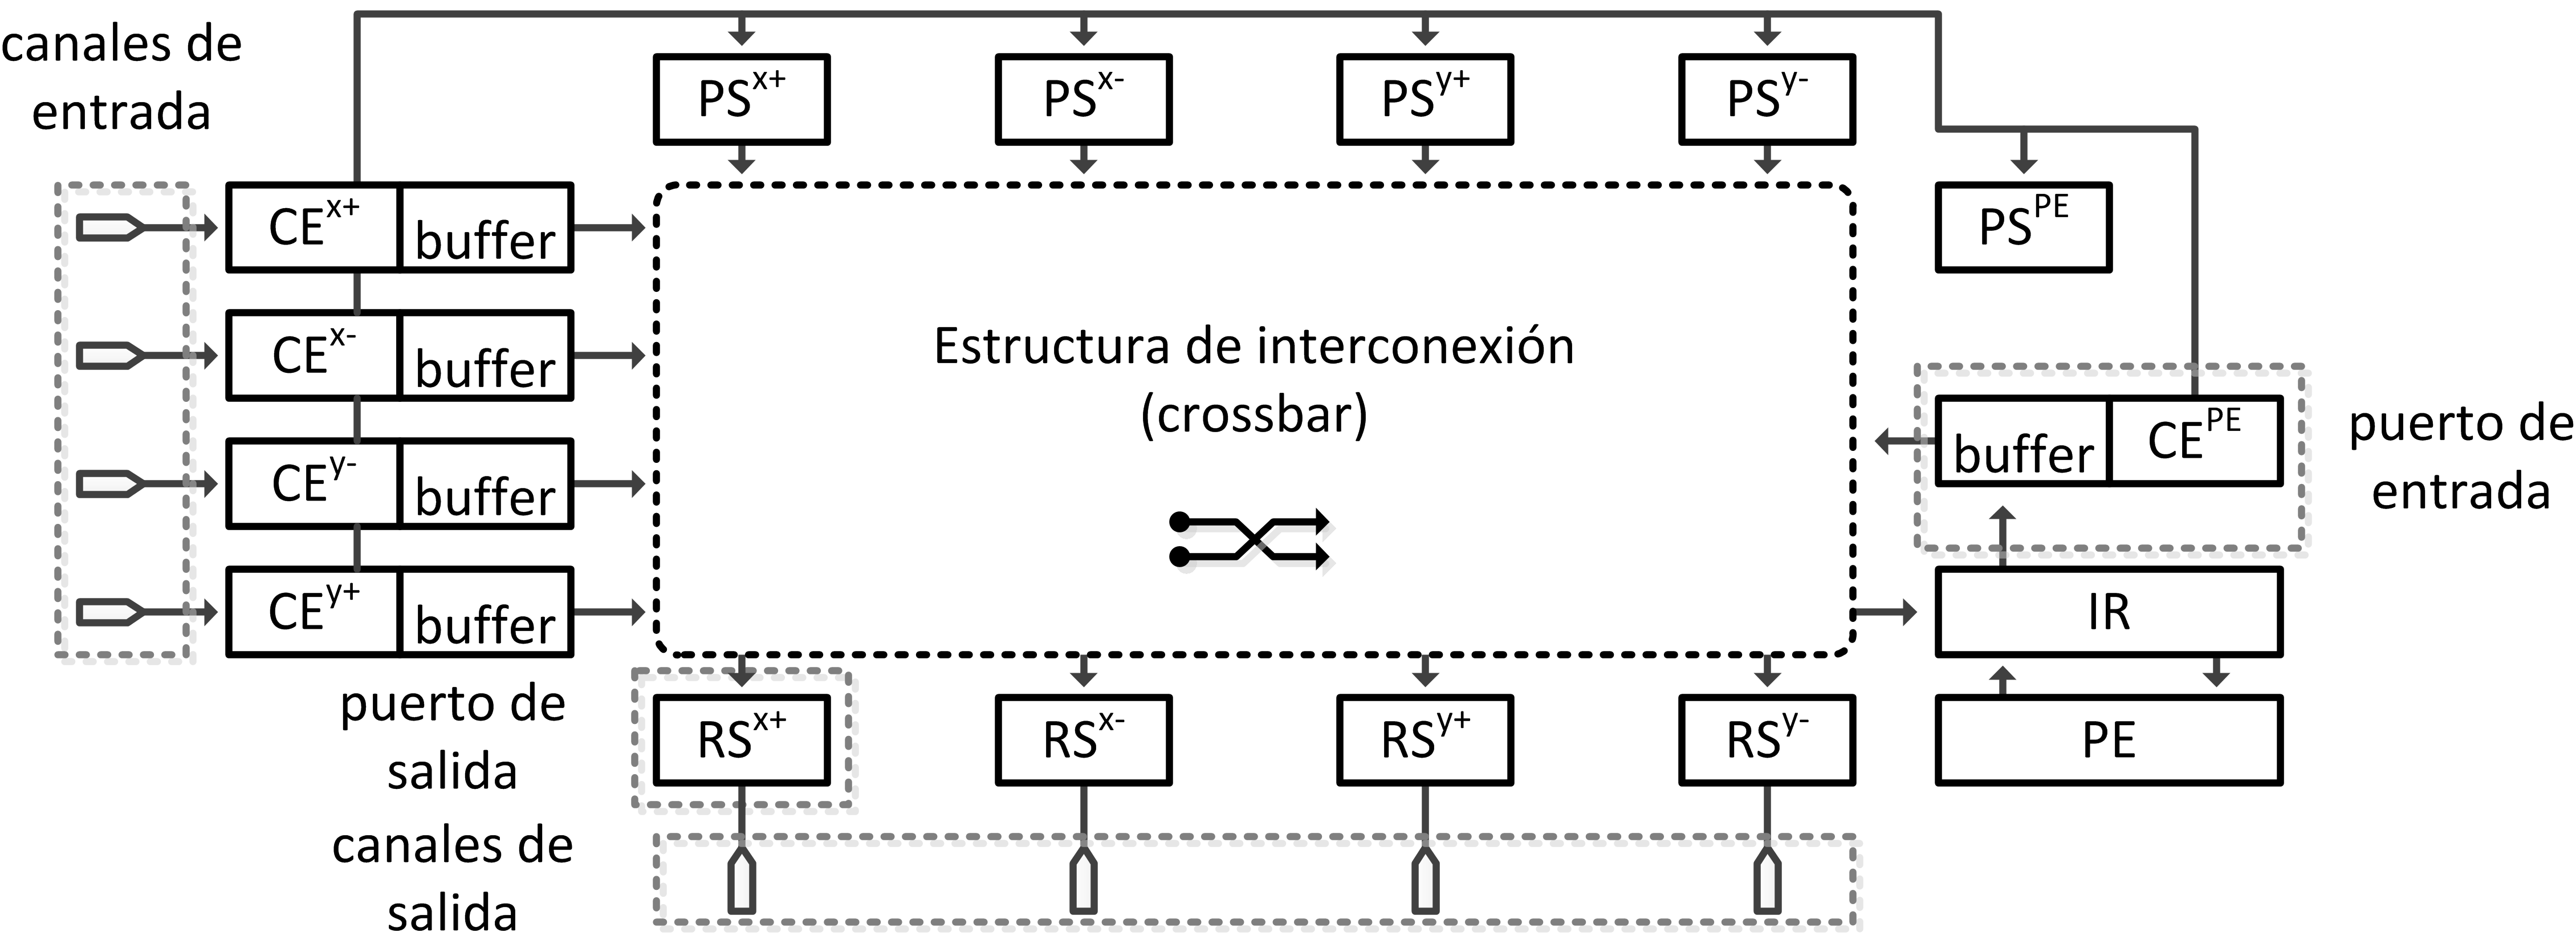
\includegraphics[width=\linewidth]{figures/ch4_top_level_router.png}
	\caption
		{	
			Diagrama a bloques del encaminador. En la figura se utilizan las siguientes abreviaciones: $CE^{w}$ módulo controlador de enlace, $PS^{w}$ módulo planificador de salida, $RS^{w}$ registro de salida, IR interfaz de red y PE elemento de procesamiento. Los paquetes ingresan a través de los canales de entrada conectados a los medios de almacenamiento temporal denominados \textit{buffers} en la figura. Los canales de salida se encuentran conectados de manera directa a los registros $RS^{w}$ del módulo.
		}
	\label{fig:ch4_top_level_router}
\end{figure}

Es importante definir los términos \textit{canal} y \textit{puerto}, ya que se utilizan para la descripción del encaminador. El término \textit{canal} se utiliza para referirse al medio físico que enlaza dos routers vecinos. El término \textit{puerto} está asociado a los modulo que se encargan de la recepción y decodificación de los paquetes entrantes a un router.

El plano de control del router está formada por bloques tipo \textit{planificador de salida} y \textit{control de enlace}. Los módulos control de enlace se encargan de la recepción de paquetes, su almacenaje en el buffer, y la liberación de solicitudes para el uso de un puerto de salida. Los bloques planificador de salida ejercen control sobre la estructura de interconexión del router, están encargados de gestionar el enlace entre un puerto de entrada con uno de los registros ligados a un puerto de salida. Los enlaces entre entradas y salidas del encaminador responden al intercambio de peticiones entre los módulos controladores de enlace y los módulos planificadores de salida.

A Partir de esta sección se utilizará de manera indiferente los términos \textit{cola} o \textit{buffer} para referirse a la estructura de almacenamiento temporal ligado a cada uno de los módulos control de enlace. De igual forma, los términos \textit{estructura de interconexión} y \textit{crossbar} se utilizan de manera indistinta para hacer referencia a la malla de interconexión entre puertos de entrada y salida del router.

\subsection{Control de enlace}\label{subsec:control_de_enlace}

El tránsito de un paquete a través del encaminador inicia con la llegada del campo \textit{identificador de cabecera} a uno de los módulos control de enlace. El flit de cabecera arrivando es almacenado al mismo tiempo que se liberan peticiones al puerto de salida requerido para continuar su avance a través de la red.

Un módulo control de enlace está organizado de manera interna en 3 bloques: una \textit{unidad de control}, un \textit{planificador de ruta} y un \textit{registro de segmentación}. La unidad de control esta encargada de generar las señales para la administración del buffer (pulso de lectura y pulso de escritura), señales para el control de flujo de datos entre encaminadores (credito de salida), y una señal de control para bloquear el resultado del proceso de cálculo de ruta de un paquete.

El bloque planificador de ruta se encarga de determinar los puertos de salida que le resultan productivos al paquete en tránsito para alcanzar su destino. El resultado del cálculo de ruta puede ofrecer múltiples opciones de puertos de salida en caso del uso de un algoritmo adaptativo o parcialmente adaptativo, sin embargo, la gestión de múltiples peticiones concurrentes a diferentes puertos de salida puede dar lugar a la duplicación de paquetes o la liberación de paquetes corruptos a la red. Para evitar el escenario anterior, se acopla un módulo \textit{selector} para limitar el número de peticiones simultáneas que puede generar el planificador de ruta de un módulo control de enlace. Los \textit{selectores} del encaminador tienen conocimiento de los puertos solicitados así como el estado actual (ocupado/disponible) de cada uno de los puertos de salida. Con el conocimiento anterior, los selectores puede dar prioridad a peticiones para puertos disponibles en ese instante, o reevaluar el estado de sus peticiones durante cada ciclo de reloj con la actualizacion de informacion acerca del estado de los puertos de salida de interes. Los modulos selector utilizan un esquema de prioridad fijo para seleccionar la petición que liberara a la red, sin embargo, esta decisión también se ve afectada por la disponibilidad de los puertos de salida. En caso de que el puerto objetivo de la solicitud de mayor prioridad no se encuentre disponible, el selector cederá el lugar a la siguiente petición cuyo puerto se encuentre receptivo a una transferencia.

Ante la captura de un nuevo paquete mientras otro se encuentra a la espera de la asignación de un puerto de salida, el control de enlace omite de manera temporal la ejecución del algoritmo de planeación de ruta y su correspondiente liberación de peticiones. Una vez que el paquete pendiente sea liberado, el control de enlace reactiva los servicios de planificación de ruta y solicitud de recursos para que el paquete en espera continúe su camino de manera normal.

Con la liberación de peticiones, el módulo control de enlace espera a la llegada de la señal \textit{pulso de transferencia}. La transición a estado alto de la señal \textit{pulso de transferencia} indica que se ha formado de manera satisfactoria un enlace entre el puerto de entrada y el puerto de salida a través del \textit{crossbar} del encaminador. 

La liberación y recepción de flits ocurre de manera independiente. En el caso que no se encuentre tráfico en la red, y el buffer de recepción se encuentre vacío, los flits pertenecientes a un paquete pueden iniciar su tránsito al puerto de salida aun cuando no se haya finalizado la recepción del total de flits pertenecientes al paquete. Este comportamiento se asemeja al modo de operación de encaminadores que utilizan la técnica \textit{wormhole} para la conmutación de paquetes.

El bloque \textit{planificador de ruta} es la implementación en hardware del algoritmo de encaminamiento. La ausencia de canales virtuales en la implementación del encaminador de este trabajo limita al uso de algoritmos determinísticos o parcialmente adaptativos. El registro al final del controlador de enlace es la única etapa de segmentado interna del encaminador. La figura \ref{fig:ch4_control_de_enlace_top} muestra el bloque controlador de enlace con sus conexiones derivadas.

\begin{figure}
	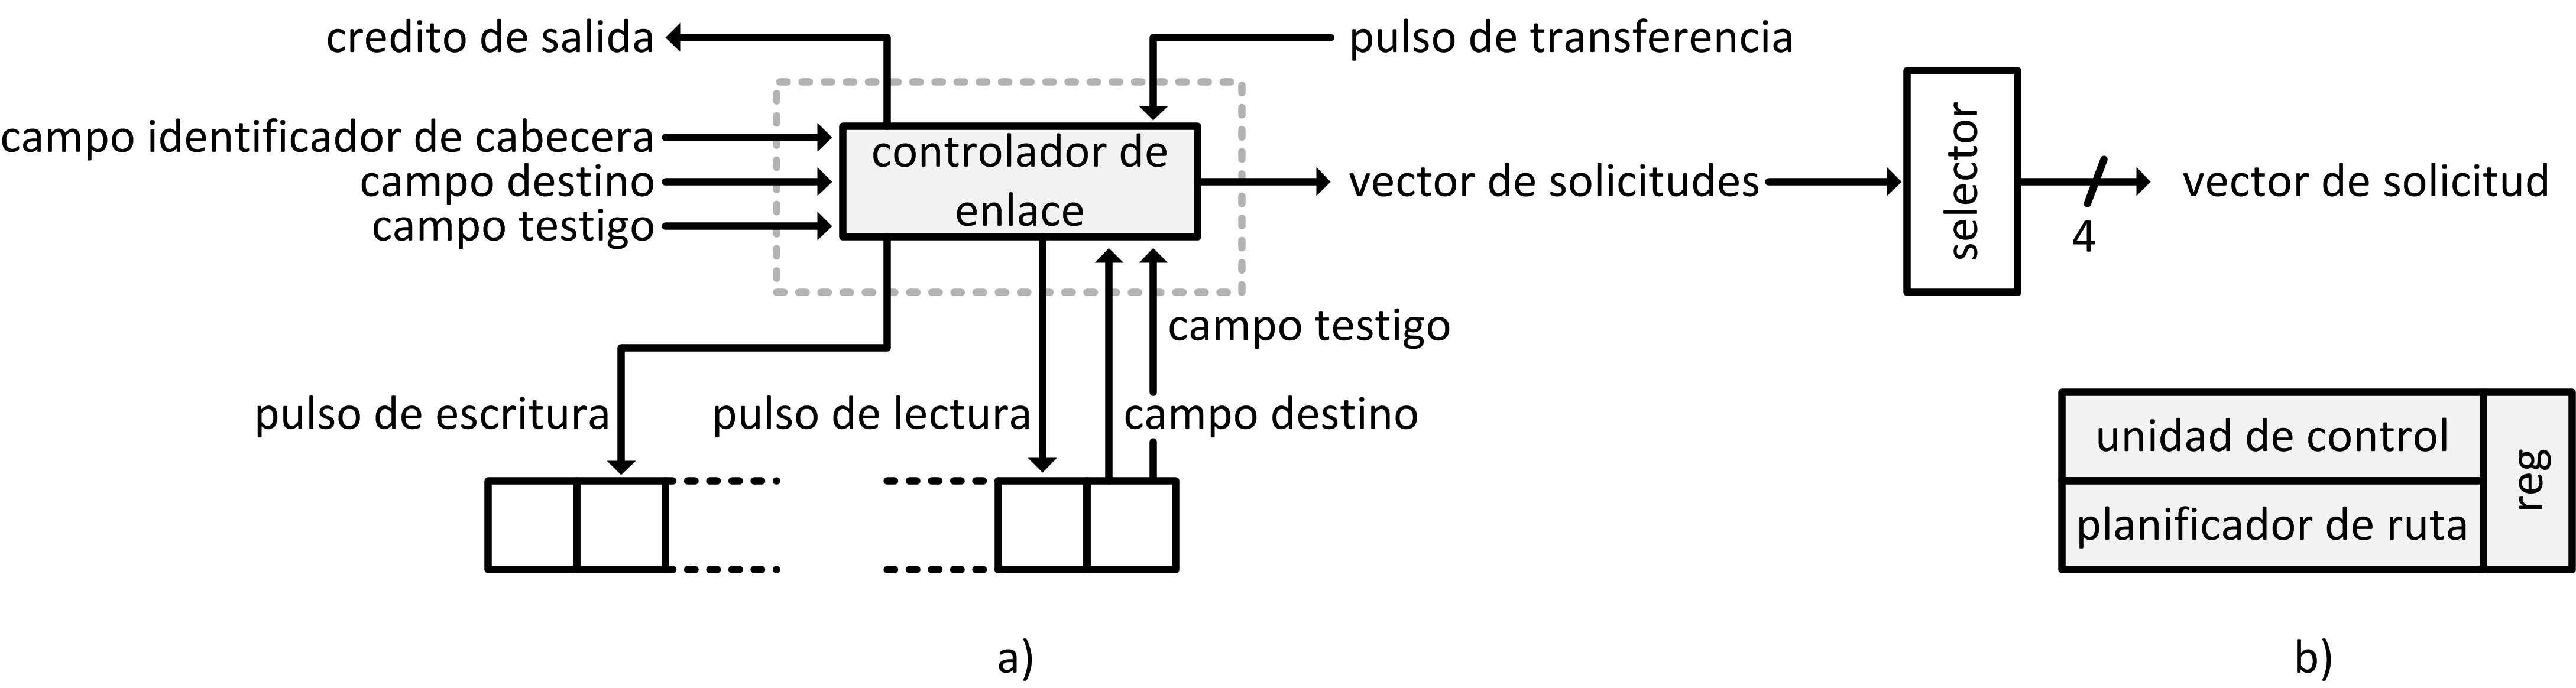
\includegraphics[width=\linewidth]{figures/ch4_control_de_enlace_top.png}
	\caption
		{	
			Los módulos control de enlace implementan la misma lógica independientemente del puerto de entrada al cual han sido asignado. La diferencia entre ellos radica en los puertos a los cuales pueden enviar peticiones. a) muestra los puertos de conexión del módulo, mientras b) hace referencia los bloques internos del mismo. 
		}
	\label{fig:ch4_control_de_enlace_top}
\end{figure}

La \textit{unidad de control} del módulo está formada por 3 máquinas de estado finito independientes. Dos de estas máquinas están dedicadas a la recepción o liberación de flits pertenecientes a un paquete. En la figura \ref{fig:ch4_fsm_control_de_enlace} se muestra el diagrama de la máquina de estados encargada de la transferencia de flits en dirección a un puerto de salida. La máquina de estados asignada a la tarea de recepción de flits utiliza el mismo esquema de transiciones entre estados, la diferencia radica en el uso del campo \textit{identificador de cabecera} para su activación y la emisión de pulsos de escritura a la \textit{cola} de almacenamiento de flits.

\begin{figure}
	\begin{center}
		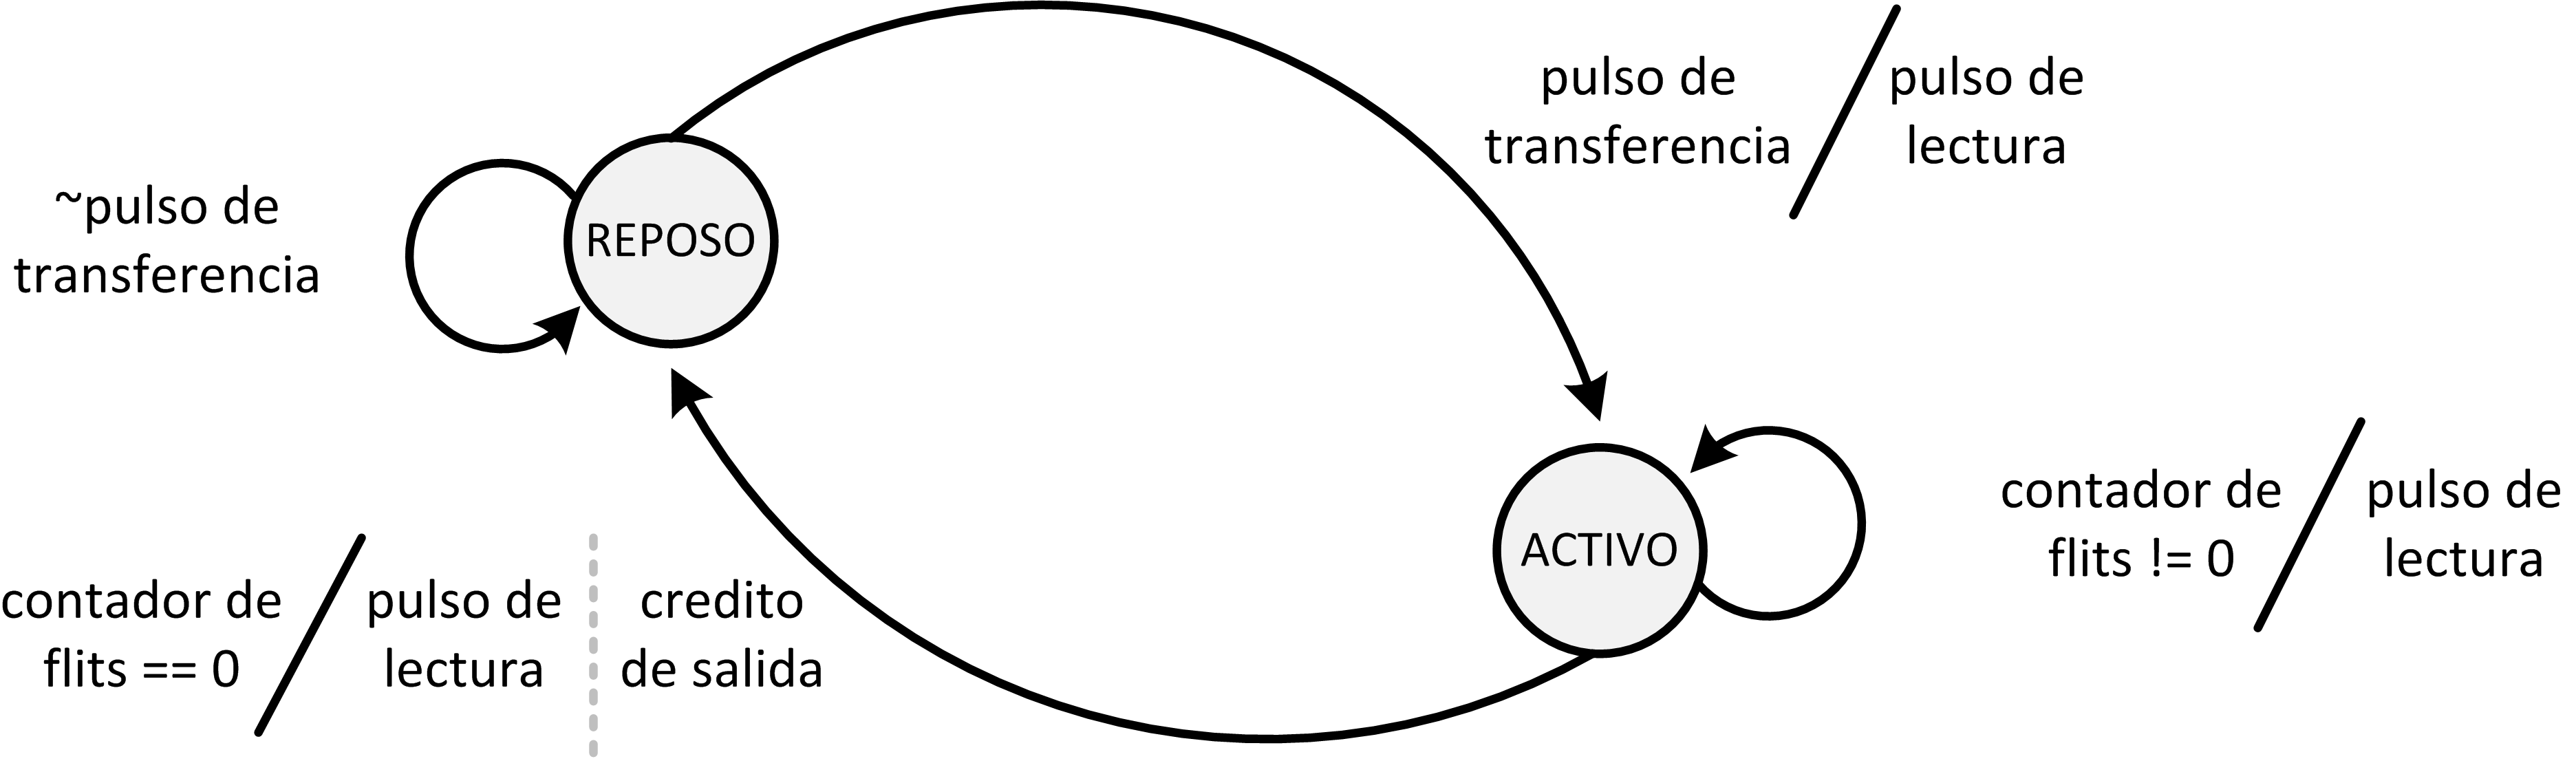
\includegraphics[scale=0.7]{figures/ch4_fsm_control_de_enlace.png}
	\end{center}
	\caption
		{	
			El uso de paquetes de longitud fija simplifica la lógica de codificación de las máquinas de estado para la recepción y transporte de paquetes entre puertos de entrada y salida. Al no contar con un flit de final de paquete, las máquinas de estado solo deben de utilizar un contador para mantener el control del inicio y fin los paquetes en tránsito. 
		}
	\label{fig:ch4_fsm_control_de_enlace}
\end{figure}

El manejo de paquetes en espera hace uso de la tercera máquina de estados y de un contador. El contador lleva registro del número de paquetes que se encuentran dentro del buffer ligado al controlador de enlace. El número de paquetes se incrementa con la transición de la máquina de estados de ingreso del estado de \textit{REPOSO} al estado \textit{ACTIVO}, mientras que el decremento del contador responde a la misma transición pero de la máquina de estados de salida.

Si el contador de paquetes se encuentra en cero, el planificador de ruta toma los campos \textit{destino}, \textit{identificador de cabecera} y \textit{testigo post-proceso} del canal de entrada e inicia el proceso de cálculo de ruta. Si el contador de paquetes es diferente a cero, el control de enlace suspende el servicio de planificación de ruta para paquetes arribando por el canal de entrada. Vale la pena notar que se considera que el contador de paquetes es diferente a cero aun cuando el único paquete dentro del control de enlace se encuentre ya en envío de sus flits al puerto de salida.

Al finalizar el desplazamiento de un paquete desde un buffer en dirección de un puerto de salida, la tercera máquina de estados verifica el número de paquetes pendientes. Si el número de paquetes en espera de recursos es mayor a cero, el proceso de planificación de ruta reinicia pero toma los campos involucrados en el proceso desde la \textit{cola} de almacenamiento de flits en lugar del canal de entrada. Para el cálculo de ruta desde el medio de almacenamiento, el campo \textit{identificador de cabecera} se vuelve innecesario ya que de antemano se conoce que el dato a la salida del buffer es un flit de cabecera.




\subsection{Planificador de salida}\label{subsec:planificador_de_salida}

Cada puerto de salida del encaminador se encuentra administrado por un módulo \textit{planificador de salida}. La tarea principal del módulo es la creación de enlaces entre puertos de entrada y salida mediante el \textit{crossbar} del router. La figura \ref{fig:ch4_planificador_de_salida_top} muestra el diagrama de un módulo planificador de salida.

El planificador de salida o simplemente \textit{planificador}, está formado por una \textit{unidad de control} y un \textit{árbitro} de peticiones. Cada planificador recibe peticiones desde puertos de entrada en direcciones opuestas al puerto de salida que administra. El trabajo de un planificador de salida inicia con la llegada de una o más peticiones desde cualquiera de los \textit{selectores} a los cuales tiene una conexión. La detección de una petición es transmitida, mediante la señal interna \textit{alguna\_peticion}, a la unidad de control del módulo. Vale la pena recordar que los selectores solo permiten la salida de una petición a la vez.

La unidad de control determina si el puerto solicitado está disponible para atender la petición en curso. A nivel del planificador la única variable que determina si un puerto de salida está habilitado para la transmisión de un paquete es la cantidad de créditos disponibles en el encaminador vecino inmediato. En este punto no se verifica si el puerto se encuentra en medio de la transmisión de un paquete, ya que este factor es evaluado en los selectores vinculados a cada módulo control de enlace. Si el puerto solicitado está disponible, la unidad de control libera un pulso para la captura del resultado del arbitraje. El arbitro del sistema es un circuito combinatorio, por esta razón los resultados del arbitraje deben de ser capturados en un registro para su uso durante todo el proceso de transferencia del paquete. El registros de captura de resultados de arbitraje no es un registro de segmentación, es un registro de estado.


La salida del planificador es un vector en codificación \smallcaps{one hot} llamado \textit{vector de configuración de crossbar}. Cada bit del vector representa uno de los puertos de entrada que pueden ser ligados al puertos de salida resguardado por el planificador. Al final de la transmisión de un paquete, el vector de configuración de crossbar transita a un estado de reposo donde todas las líneas de comunicación entre el puerto de salida y el encaminador vecino se mantienen en estado bajo. Mantener las líneas en estado bajo entre encaminadores cuando no hay paquetes en transito resulta fundamental, ya que la detección de un nuevo paquete se lleva a cabo mediante el sensado del cambio de estado del campo \textit{identificador de cabecera}. La presencia de perturbaciones en un canal de comunicación entre encaminadores puede resultar en la generación de paquetes espurios o la corrupción de paquetes en tránsito a través de la red.

\begin{figure}
	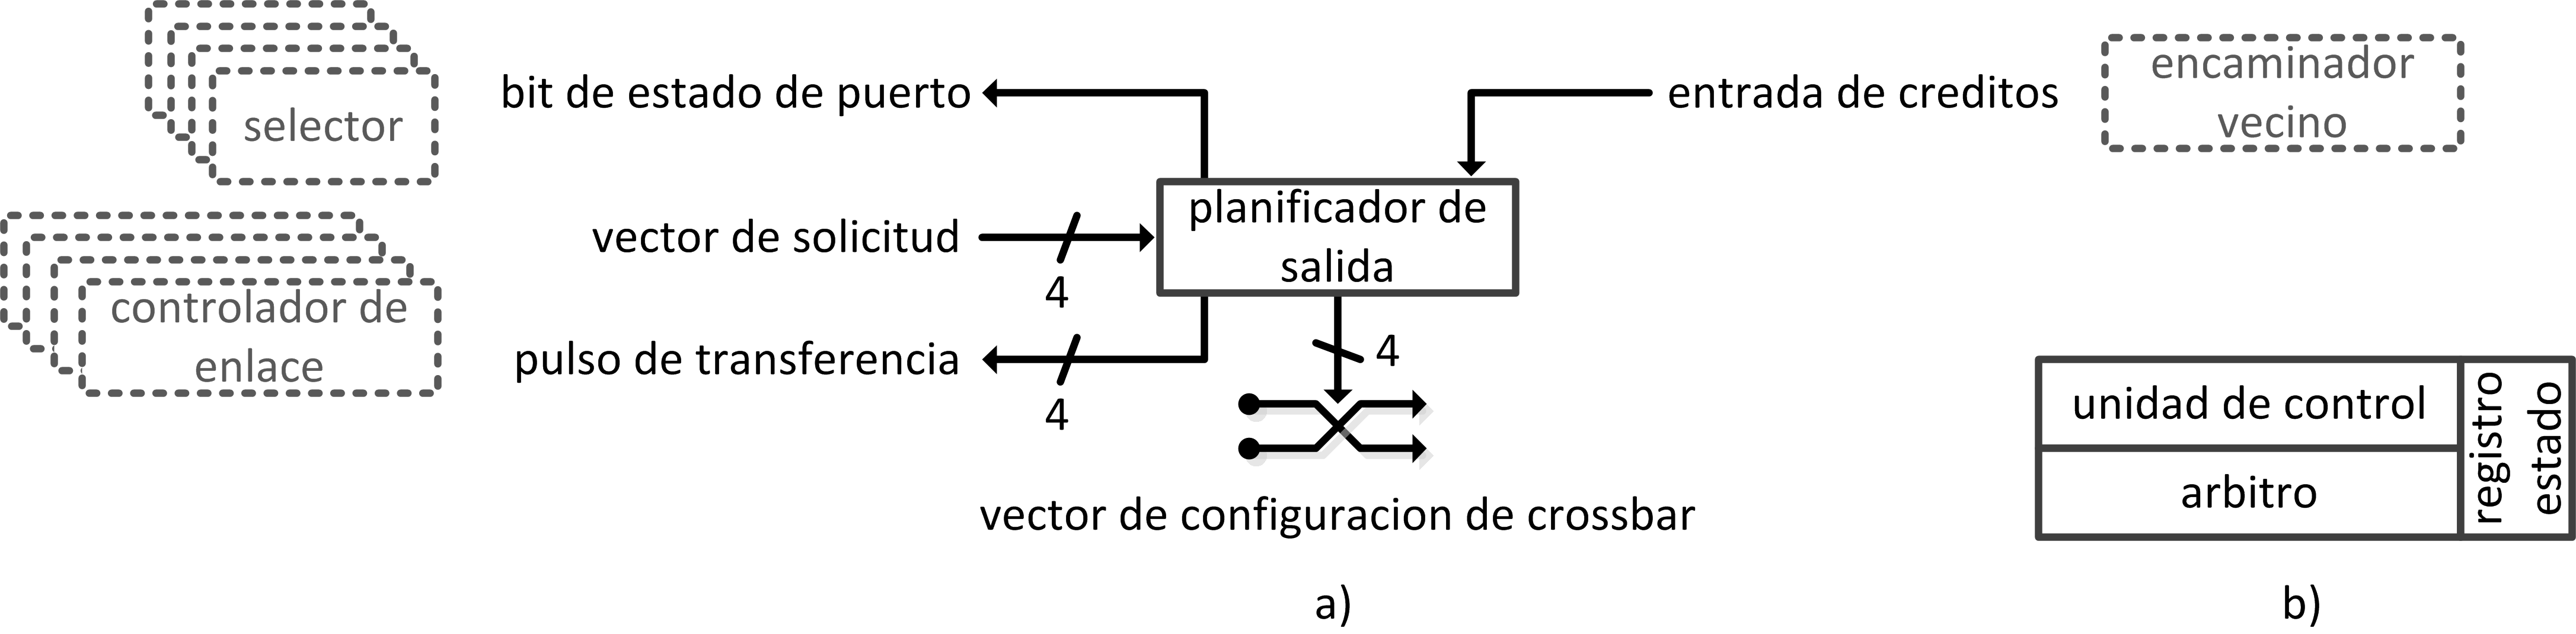
\includegraphics[width=\linewidth]{figures/ch4_planificador_de_salida_top.png}
	\caption
		{	
			El módulo planificador de salida se conecta a los módulos \textit{controlador de enlace} y \textit{selector} de los puertos de entrada en direcciones opuestas al puerto de salida que resguarda. a) muestra las conexiones entre un planificador de salida y los demás módulos del encaminador. b) presenta los bloques que conforman a un planificador de salida.
		}
	\label{fig:ch4_planificador_de_salida_top}
\end{figure}

Una vez terminado el proceso de arbitraje, el módulo planificador de salida debe de notificar al \textit{controlador de enlace} ganador que se ha formado un vínculo de manera satisfactoria, y que es tiempo de iniciar la transferencia de flits desde el buffer del puerto de entrada al puerto de salida. El vector \textit{pulso de transferencia} se encuentra conectado a todos los módulos control de enlace relacionados con el planificador. Este vector utiliza como máscara la señal \textit{vector de configuración de crossbar} para propagar solo al módulo ganador la señal de inicio de transferencia.



\subsection{Camino de datos}\label{subsec:camino_de_datos}

El camino de datos del router está formado por los buffers empotrados en cada puerto de entrada, el medio de interconexión entre puertos, y los registros de cada uno de los puertos de salida.

El medio de interconexión entre puertos está implementado como una estructura tipo \textit{crossbar}, la cual permite conexiones simultáneas entre puertos. El crossbar está descrito como un conjunto de multiplexores que permiten el paso de una fuente de datos dependiente de una señal de control. La arquitectura a alto nivel del camino de datos se muestra en la figura \ref{fig:ch4_camino_de_datos}.

\begin{figure}
	\begin{center}
		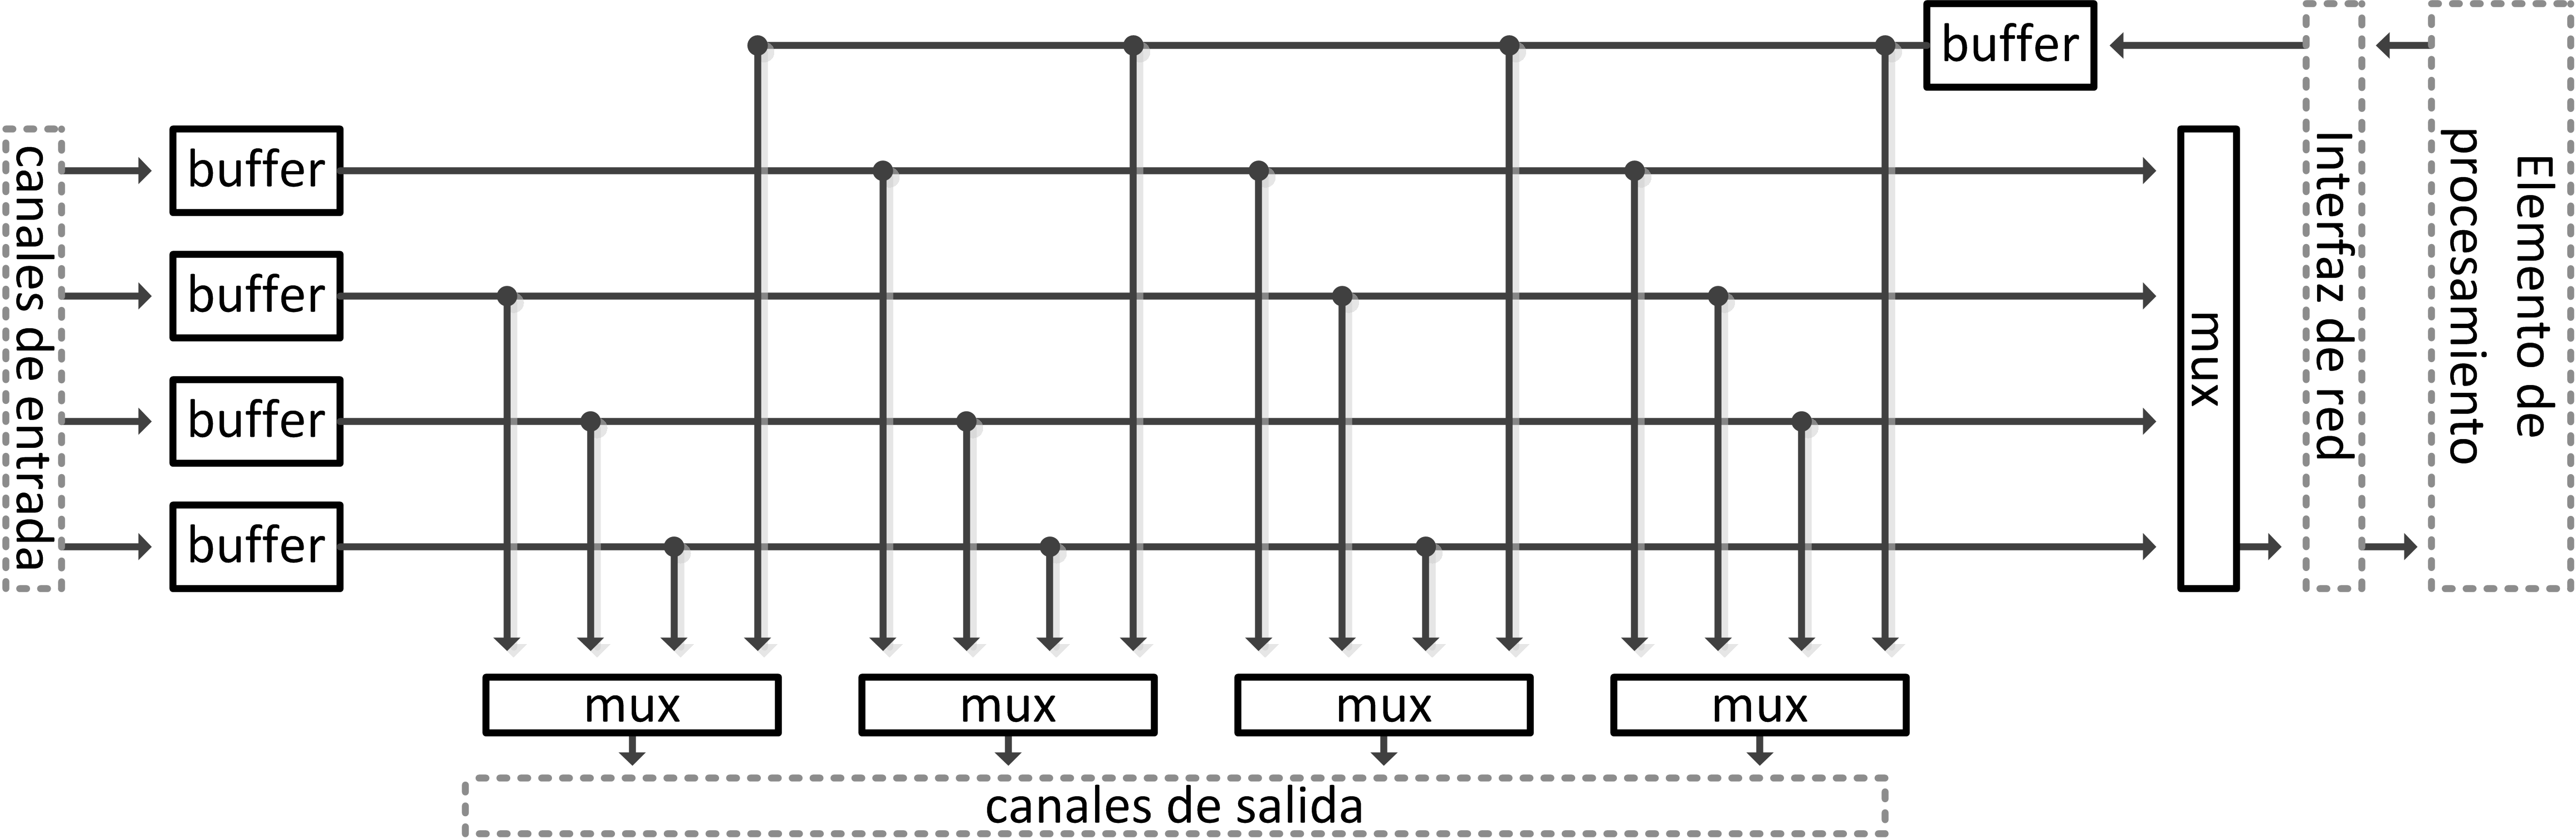
\includegraphics[scale=0.6]{figures/ch4_camino_de_datos.png}
	\end{center}
	\caption
		{	
			Los multiplexores del \textit{camino de datos} están controlados por la señal \textit{vector de configuración de crossbar} proveniente de los planificadores de salida. El manejo de \textit{buffers} está a cargo de los controladores de enlace.
		}
	\label{fig:ch4_camino_de_datos}
\end{figure}

Es importante notar la simetría de todos los canales de entrada/salida del encaminador, incluyendo el puerto en dirección del elemento de procesamiento. En la etapa de diseño se decidió por esta estructura homogénea en lugar de integrar fuertemente la interfaz de red con el puerto al elemento de procesamiento, de esta manera se provee un diseño más versátil al momento de la conexión de diferentes unidades funcionales.


\section{Interfaz de red}\label{sec:encaminador_de_red}

Los paquetes de información en tránsito a través de la red utilizan el formato descrito en la sección \ref{sec:formato_de_paquetes}. El formato fue diseñado en orden de simplificar el hardware necesario para la decodificación y transporte de información a través de la red, tomando en cuenta las restricciones físicas que impone el ancho de canal entre routers. Sin embargo, la información contenida en el paquete debe ser pre-procesada antes de ser inyectada a un elemento de procesamiento.

La tarea del desempaquetado de información se lleva a cabo en las interfaces de red de cada nodo. La figura \ref{fig:ch4_interfaz_de_red_top} muestra el diagrama a bloques general de una interfaz de red.

El encaminador del nodo interactúa con la interfaz de red como si se tratase de un encaminador vecino. La transferencia de información entre la interfaz de red y el encaminador se basa en el intercambio de paquetes y la entrega/recepción de créditos para mantener el control sobre el flujo de información.


\begin{figure}
	\begin{center}
		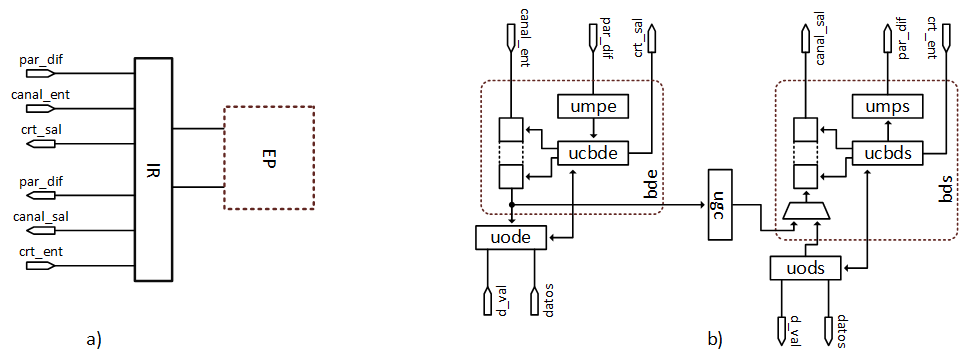
\includegraphics[scale=0.6]{figures/ch4_interfaz_de_red_top.png}
	\end{center}
	\caption
		{	
			Interfaz de red. a) la interfaz de red se conecta al encaminador como un vecino más de la red. b) modelo general de interfaz de red. Los tamaño de palabra y protocolos de comunicación utilizados por el elemento de procesamiento modelan las líneas de transferencia de información con la interfaz de red.
		}
	\label{fig:ch4_interfaz_de_red_top}
\end{figure}

El elemento de procesamiento define las señales de control y datos involucrados en la interacción con la interfaz de red. El área de intercambio entre interfaz y elemento de procesamiento representa un desafío para la versatilidad de la red, ya que diferentes elementos de procesamiento requerirán interfaces de red a medida. Para facilitar la tarea de diseño de interfaces se ha dividido internamente el módulo en bloques de entrada y salida como se muestra en la figura \ref{fig:ch4_interfaz_de_red_top} \textit{b)}.

La áreas de interacción con el encaminador no requieren un análisis profundo ya que utilizan la misma filosofía de envío/recepción de paquetes entre routers, y de hecho, reutilizan los mecanismo de manejo de paquetes utilizados por los módulos \textit{control de enlace} y \textit{planificador de salida} presentados en la sección \ref{sec:encaminador_de_red}. En especifico, el mecanismo utilizado es el mismo implementado en la máquinas de estado empotrada en la unidad de control del módulo \textit{control de enlace}.


EL bloque de entrada de la interfaz provee los datos de trabajo para el elemento de procesamiento, además de al menos una señal de control para indicar que los datos a la entrada del elemento de procesamiento son válidos y puede iniciar la transformación de la información. Es trabajo del bloque de entrada reorganizar los flits de datos de un paquete de manera que se presenten en el formato nativo de trabajo del elemento de procesamiento, además de cumplir con cualquier protocolo de transferencia de información impuesto por este último.

Por su parte, el bloque de salida espera la finalización del trabajo llevado a cabo por el elemento de procesamiento. Una señal de control o una transacción de un protocolo de comunicación (\textit{handshake}) indica al bloque de salida que los datos son válidos y puede iniciar la captura de resultados. Los datos transmitidos por el elemento de procesamiento pueden encontrarse en tamaños de palabra diferentes a los de un flit, por lo que es tarea del bloque de salida reorganizar la información de manera que puedan empaquetarse previo a su liberación a la red.

El flit de cabecera no se envía al elemento de procesamiento, todo el trabajo de re-codificación de la información de la cabecera se lleva a cabo dentro de la interfaz de red. De manera ordinaria, el tratamiento que se le da a un flit de cabecera consiste en asignar el estado alto a su campo \textit{testigo post-proceso} y el intercambio de los campos \textit{destino} y \textit{puerta}. Los cambios al flit de cabecera ocasionan que el paquete viajando con los resultados no compita nuevamente por el uso de un elemento de procesamiento en ningún otro nodo de la red, además, su nueva dirección destino es una de las puertas de salida de la red.


\subsection{Caso de estudio: encriptador DES}\label{subsec:caso_de_estudio_encriptador_des}

En esta sección se presenta el desarrollo de una interfaz de red para un bloque encriptador basado en el algoritmo DES \cite{chapter0:NIST:1977:DES}. El encriptador trabaja con dos bloques de 64 bits de datos, un conjunto de datos a encriptar y una clave de cifrado. El estándar de encriptación DES especifica el uso de claves de longitud de 56 bits, sin embargo, es una práctica común el agregar 1 bit de paridad por cada byte que conforma la clave. El bit de paridad sirve para verificar la integridad de la clave de encriptación.
El elemento de encriptación recibe la frase original y la clave de cifrado en forma de una carga paralela como se muestra en la figura \ref{fig:ch4_interfaz_des}. La señal \textit{pulso de inicio} se utiliza para indicar al encriptador que los datos en sus puertos de entrada son válidos y puede iniciar con su tarea.

Como resultado, el módulo DES regresa una palabra de 64 bits conteniendo la información cifrada. Se utiliza la señal \textit{pulso de término} para indicar a la interfaz de red que los datos en el puerto de salida del encriptador son válidos para su captura. Para complementar el control de flujo de información entre la interfaz de red y el encriptador se agrega la señal de control \textit{elemento ocupado}.


\begin{figure}
	\begin{center}
		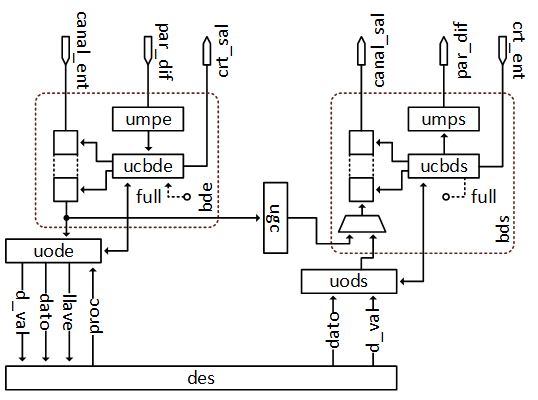
\includegraphics[scale = 0.8]{figures/ch4_interfaz_des.png}
	\end{center}
	\caption
		{	
			Las líneas de comunicación entre interfaz y elemento de procesamiento están definidas para acoplarse al formato utilizado por el elemento funcional. En este ejemplo se favorece una interfaz con de carga paralela de datos.
		}
	\label{fig:ch4_interfaz_des}
\end{figure}

Más a detalle, el bloque de entrada está compuesto por un banco de registros y una unidad de control. El encriptador requiere que se alimente con los datos de trabajo de forma paralela, por lo tanto, cada registro del banco tiene un puerto de salida exclusivo. El bus de datos de entrada del encriptador consta de dos palabras de 64 bits, por lo cual, suponiendo flits de 32 bits, se deduce que cada paquete de la red debe de estar formado por un flit de cabecera y 4 flits de datos.

El trabajo del bloque de entrada, mostrado en la figura \ref{fig:ch4_bloque_entrada_des}, inicia con la detección del campo \textit{identificador de cabecera}, este dispara la rutina de captura de flits de la red. El tamaño del paquete (5 flits) se a especificado de manera previa a la síntesis del acelerador, por lo que el bloque de entrada conoce de antemano el número de flits a capturar por paquete. Con la captura de todos los flits de un paquete, la unidad de control libera la señal \textit{pulso de inicio} para indicar al encriptador que en sus puertos de entrada se encuentra un conjunto de datos válidos para su cifrado.


\begin{figure}
	\begin{center}
		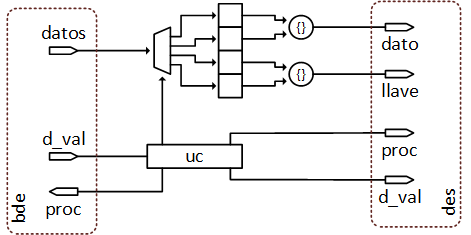
\includegraphics[scale=0.6]{figures/ch4_bloque_entrada_des.png}
	\end{center}
	\caption
		{	
			Las líneas de comunicación entre interfaz y elemento de procesamiento están definidas para acoplarse al formato utilizado por el elemento funcional. En este ejemplo se favorece una interfaz con de carga paralela de datos.
		}
	\label{fig:ch4_bloque_entrada_des}
\end{figure}

Con el retorno a estado bajo de la señal \textit{pulso de inicio} se asume que el encriptador a tomado los datos necesarios para su trabajo, por lo tanto el bloque de entrada esta en la libertad regresar un credito al router y aceptar un nuevo paquete de datos. El caso descrito en los párrafos anteriores refleja el mejor escenario donde el elemento de procesamiento se encuentra disponible y no se encuentran paquetes encriptados a la espera de su liberación a la red. En caso de tener al encriptador en medio de una operación (señal \textit{elemento ocupado}), o tener paquetes a la espera en el bloque de salida (señal \textit{cero créditos}), la unidad de control del bloque de entrada es capaz de capturar un paquete, sin embargo no podrá dar la señal de \textit{pulso de inicio} hasta que el elemento de procesamiento esté libre y se cuente con espacio para almacenar el resultado del cifrado. El numero de creditos que se debe de asignar al módulo \textit{planificador de salida} encargado de las comunicaciones con la interfaz de red debe de reflejar la capacidad de almacenamiento de esta última. En este ejemplo en particular, la interfaz de red solo tiene la capacidad de retener de manera temporal un paquete, si se asigna un número mayor de créditos del lado del encaminador se corre el riesgo de sufrir pérdida de paquetes por la sobre utilización del banco de registros de la interfaz.


El bloque de salida de la interfaz de red está formado por un par de registros, uno para contener el resultado de la transformación del flit de cabecera y un segundo registro para almacenar los datos cifrados por el encriptador. El registro para el flit de cabecera tiene una longitud de 32 bits mientras que el registro de datos cifrados tiene un tamaño de palabra de 64 bits. Además de los registros, el bloque de salida contiene un multiplexor que desemboca al canal de salida de la interfaz de red, y una unidad de control para formar los paquetes previo a su liberación a la red. El diagrama del bloque de salida se presenta en la figura \ref{fig:ch4_bloque_salida_des}.

\begin{figure}
	\begin{center}
		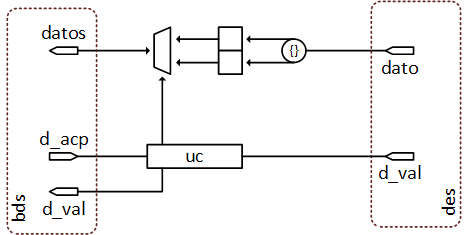
\includegraphics[scale=0.7]{figures/ch4_bloque_salida_des.png}
	\end{center}
	\caption
		{	
			Bloque de salida de la interfaz de red para el encriptado DES. La unidad de control utiliza un mecanismo similar al de los módulos \textit{control de enlace} para liberar el paquete desde su medio de almacenamiento interno.
		}
	\label{fig:ch4_bloque_salida_des}
\end{figure}

La señal de control \textit{pulso de término} indica al bloque de salida que la operación del encriptador a terminado, y que los datos presentes en su puerto de salida serán válidos por el resto del ciclo de reloj. En respuesta a esta última señal, el bloque de salida captura en sus registros internos el resultado generado por el encriptador e inicia el proceso de liberación del paquete a la red.


La operación de transmitir un paquete cifrado al encaminador del nodo se lleva a cabo de la siguiente manera: En primer lugar se verifica que se cuente con al menos un crédito disponible para la transferencia del paquete, de así serlo, la unidad de control entra en un ciclo para liberar un paquete iniciando con el flit de cabecera modificado, después se transmite la parte alta del registro donde se almacenaron los 64 bits de la palabra cifrada y por último se libera la parte baja del mismo registro. Hasta el momento se han liberado 3 flits, sin embargo los paquetes de red están formados de 5 elementos, por lo que la unidad de control libera dos flits vacíos para generar un paquete válido para la red. En caso de no contar con créditos disponibles, el bloque de salida retiene el resultado de la última ejecución del encriptador y deja saber al bloque de entrada, mediante la señal \textit{cero créditos}, que no es posible seguir aceptando nuevos paquetes hasta recibir créditos del router.